\chapter{Domain Problem Characterization}
\label{chap:problem}

In order to clearly understand the problems faced by the healthcare professional in interpreting the gameplay into a meaningful therapy routine, first it is important to have an understanding of how the game is played. Based on this understanding, then it will be possible to find out what kind of information needed by defining questions usually asked by the users. In the end, visualization requirement elicitation will be done by translating each question into list of tasks. This chapter discusses each one of these steps in details.

\section{Hammer and Planks Game Dynamics}

Played with Kinect, it is possible to play Hammer and Planks in three different ways:
\begin{enumerate}
  \item BodyTilt:
  Player puts both arm in his/her hips and move the the upper body (from the waist up) to the right, left, forward or backward to navigate the boat(figure \ref{fig:movement_type} (left)). 
  \item HandPoint:
  Player lifts one of his/her forearm in front of the body with the palm facing forward. Navigating the boat can be done by moving the forearm to the right, left, forward, or backward(figure \ref{fig:movement_type} (right)).
  \item ShoulderCGE:
  Player lifts one of his/her arm in front of the body and bend the elbow. Moving the elbow up and down will navigate the boat up and down the screen.
\end{enumerate}

For both the BodyTilt and HandPoint there are three direction available: (i) Horizontal: the screen scrolls from top to bottom and player navigates the ship from left to right (ii) Vertical: the screen scrolls from right to left and player navigates the ship from top to bottom of the screen(iii) Both: the screen scrolls from top to bottom and player navigates the ship from left to right. He/she can also move the boat faster or slower by bending the upper body (BodyTilt) or arm (HandPoint) forward or backward . For ShoulderCGE there is only vertical direction. In this thesis, I only interested in games played using BodyTilt and HandPoint movement for both direction since the information generated are richer, thus harder for the specialist to understand.

%\begin{figure}
%\centering
%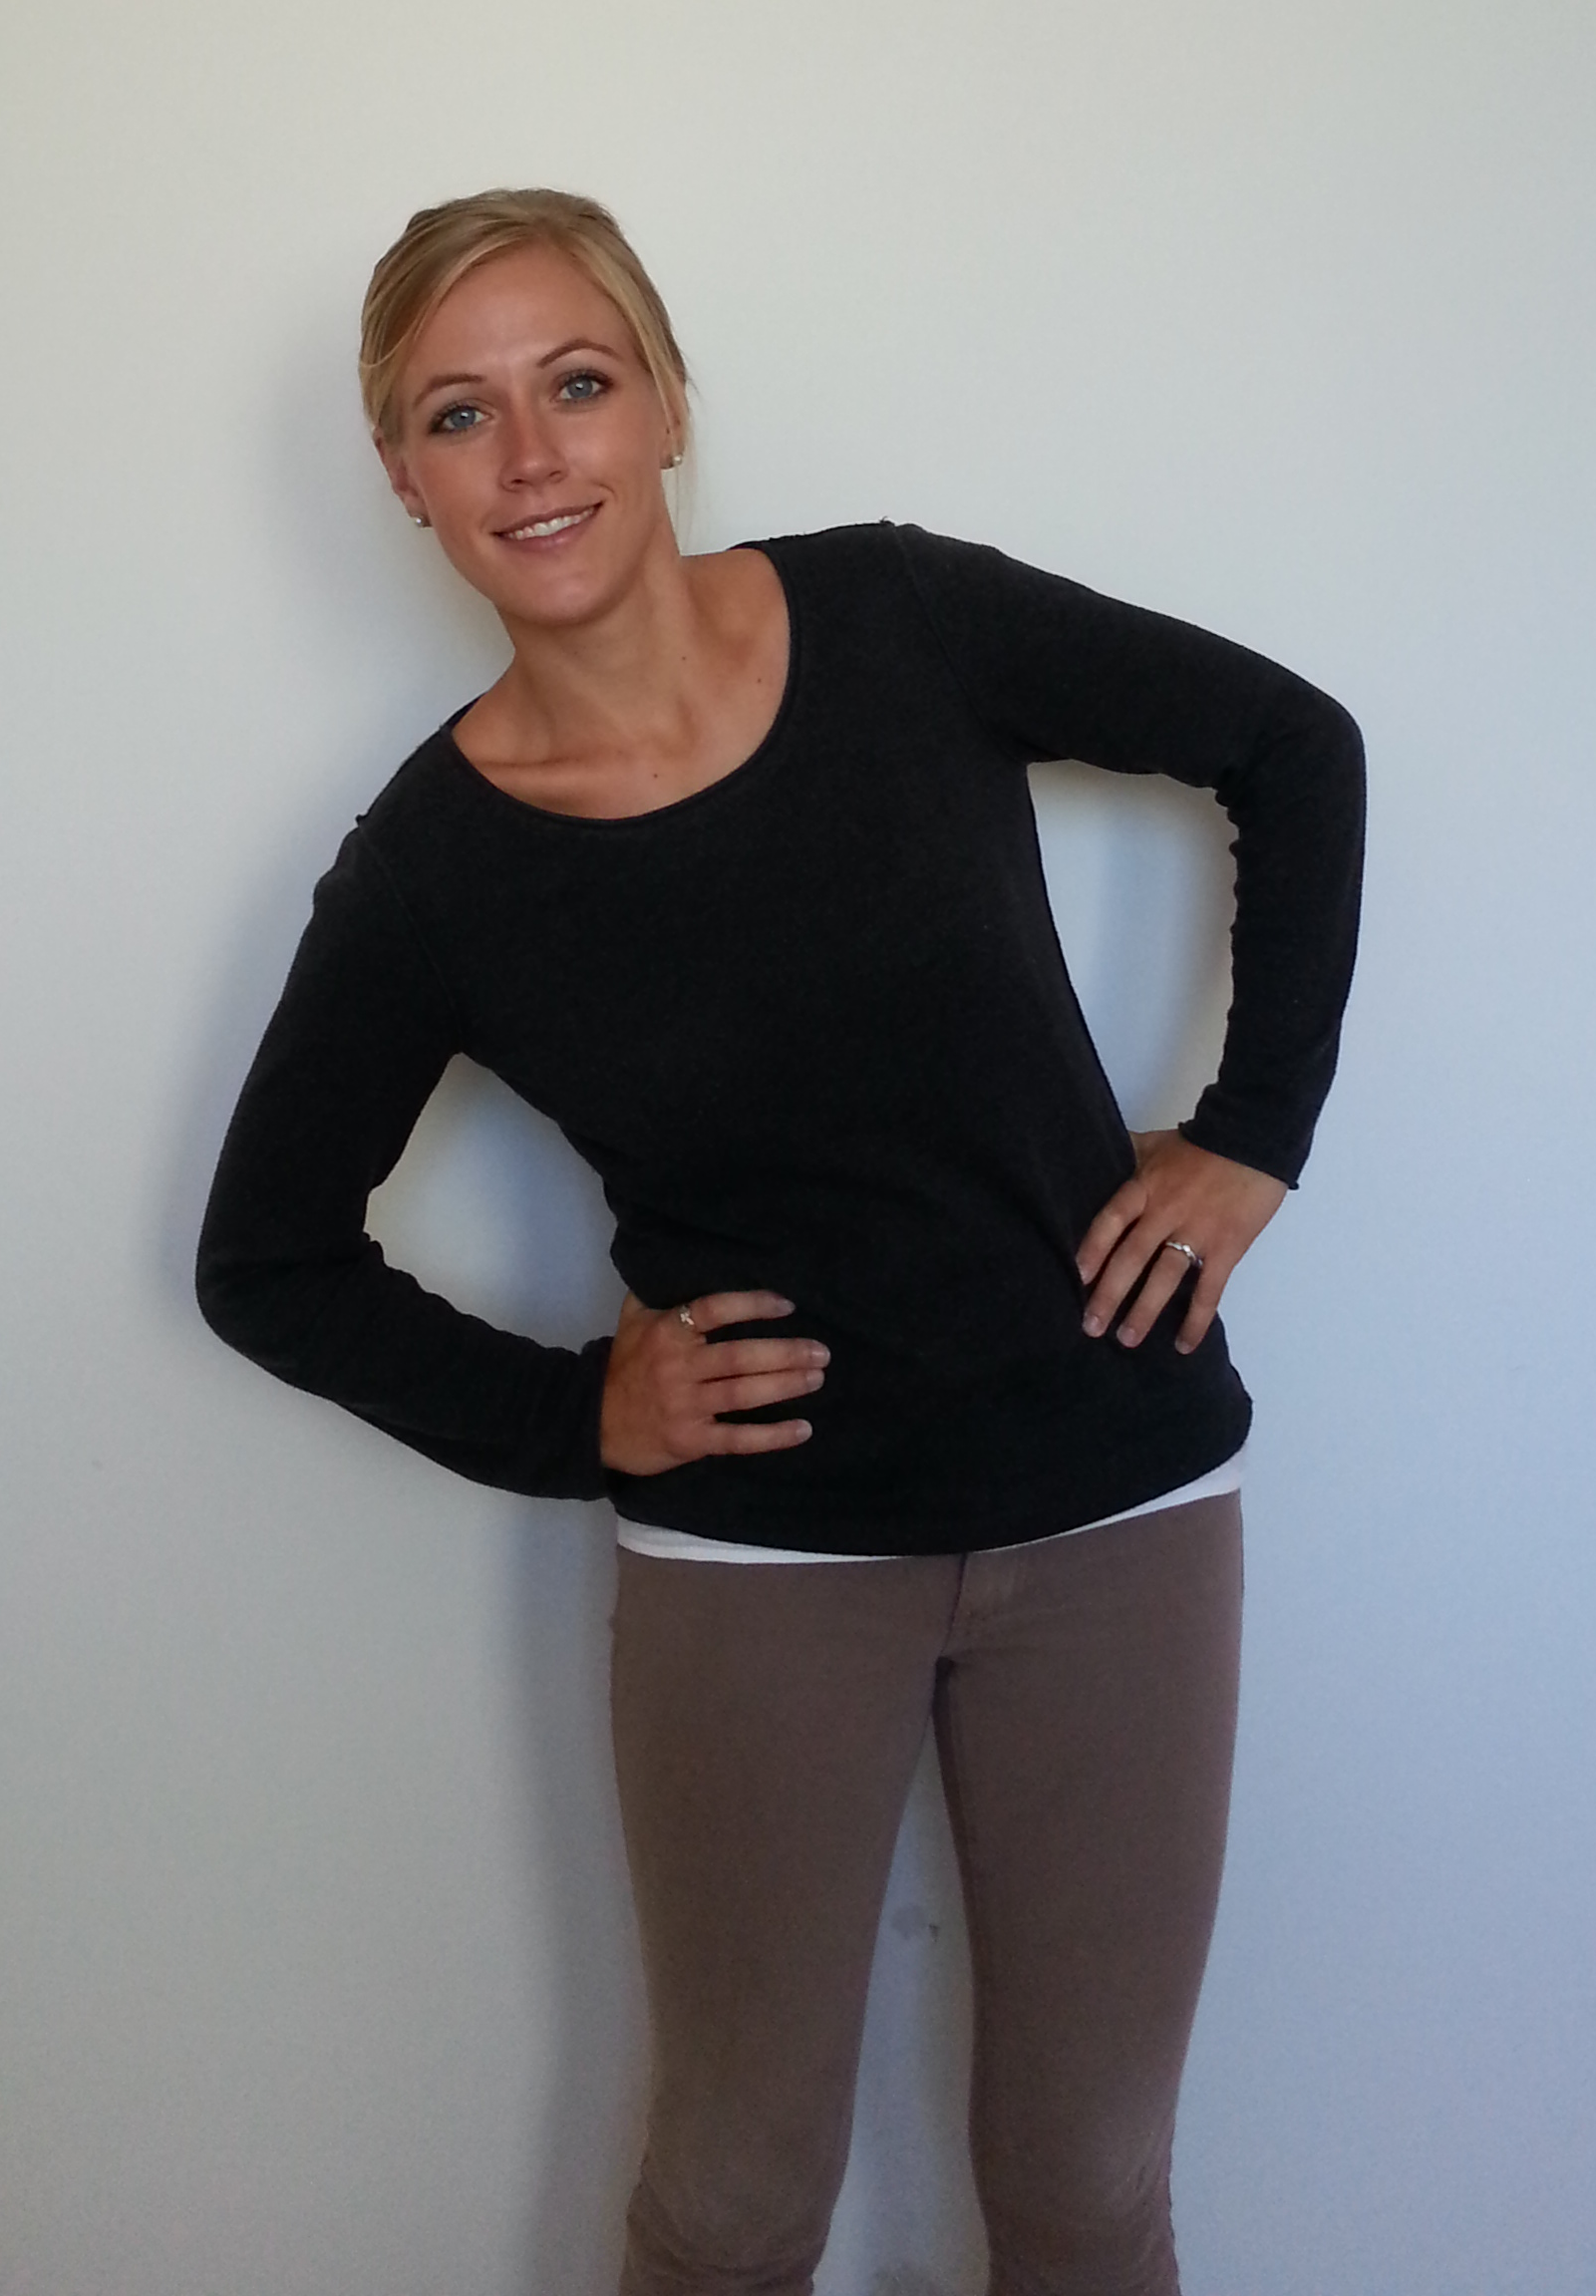
\includegraphics[width=110mm]{mia_bodytilt.png}
%\caption{BodyTilt \label{overflow}}
%\end{figure}

\begin{figure}%
    \centering
    \subfloat[BodyTilt]{{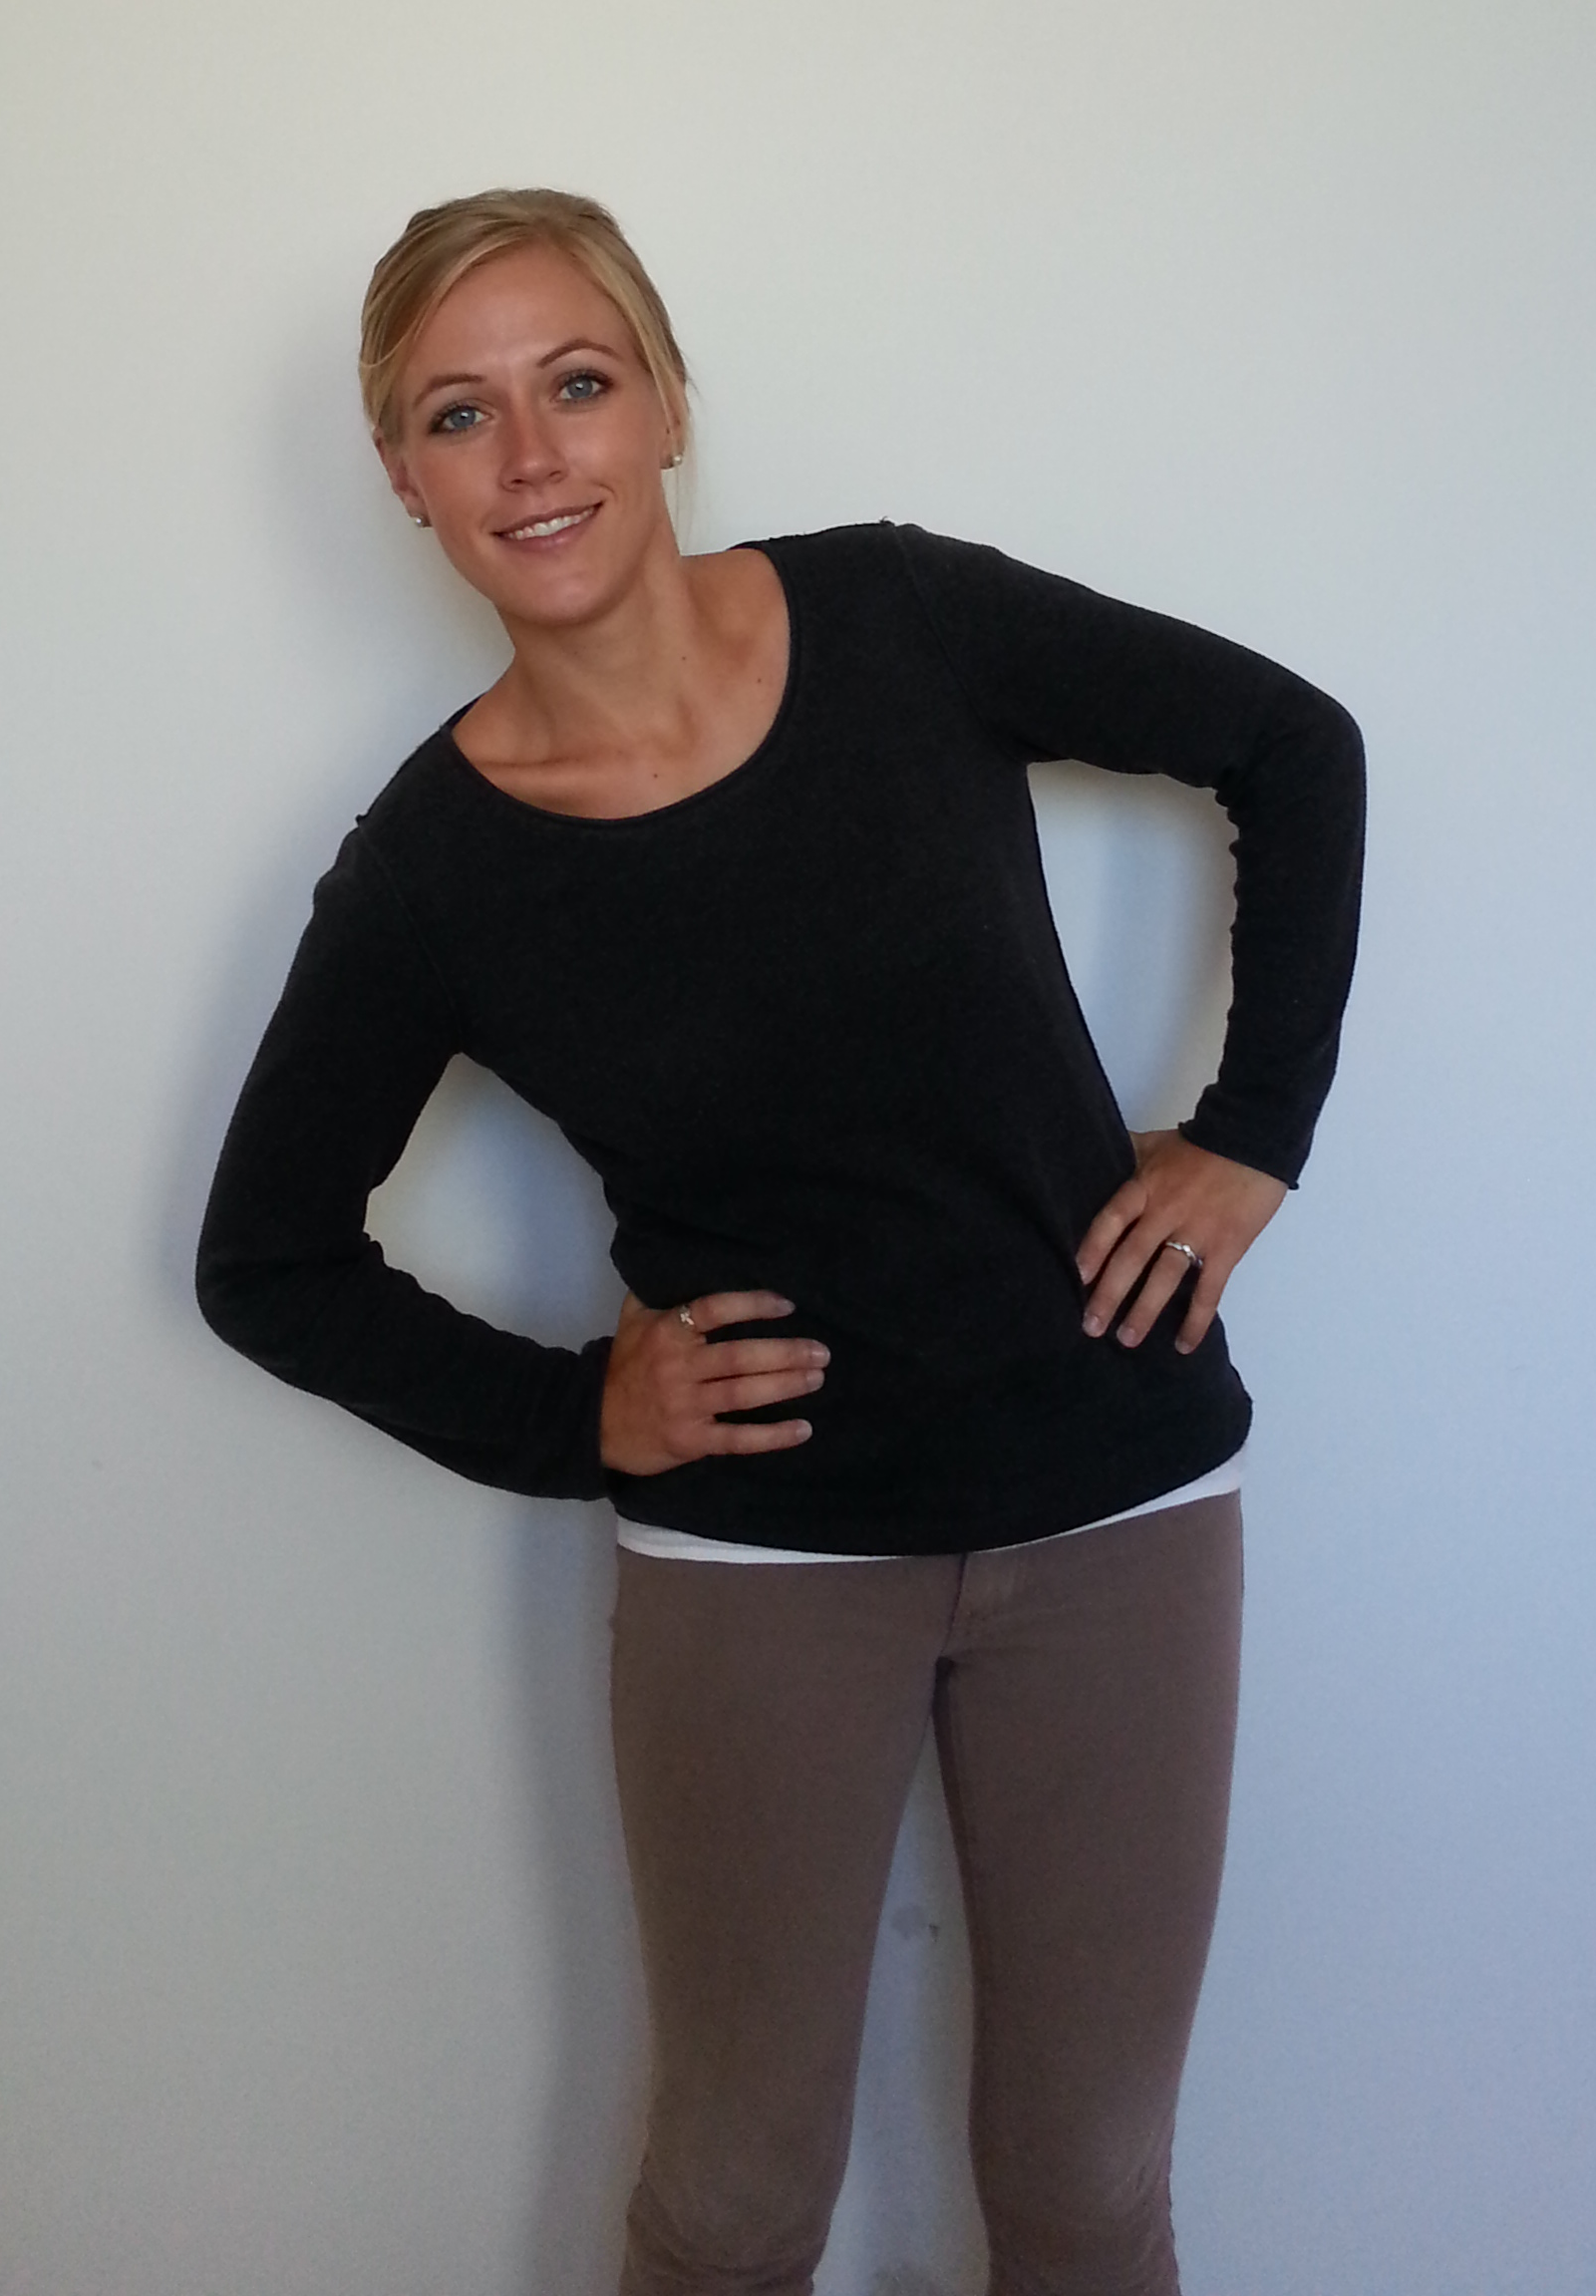
\includegraphics[width=5.5cm]{mia_bodytilt.png} }}%
    \qquad
    \subfloat[HandPoint]{{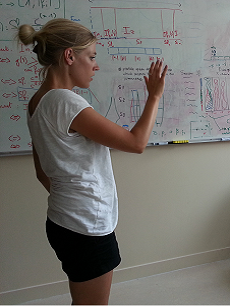
\includegraphics[width=5.5cm]{mia_handpoint.png} }}%
    \caption{Hammer and Planks movement type}%
    \label{fig:movement_type}%
\end{figure}


Before each session, the healthcare professionals will set the number of objects (enemies, bonuses, obstacles), activity duration and repetition, as well as area in which the objects can appear. Therefore he can adjust the difficulty of the game for different session.


\section{Target User Questions}

A traditional Hemiplegic therapy routine usually involved the therapist ordering a patient to perform several movement repetitively \cite{rahman}. By the end of the session, the therapist will analyse how the patient has performed based on the quality of movement as well as how the patient has progressed compared to the previous session. Based on this analysis, the therapist will then configure a new routine to further the patient's progress, if needed.

However, by using a game to facilitate the therapy, it is difficult to monitor how often the patient has moved his/her arm, to which direction and to which objects this movement is associated. Based on this reason, I identified 5 types of questions usually inquired:

\newcommand{\subscript}[2]{$#1 _ #2$}	
\begin{enumerate}[label=(\subscript{Q}{\arabic*})]
\item For a given session, to which direction (right/left) the player moved more? \label{q1}
\item For a given session, how does the player perform based on the number of objects collected, avoided, or killed with respect to the area of the movement?\label{q2}
\item For a given session, how does the player perform based on the number of objects collected, avoided, or killed with respect to the area of movement and the speed in which the game is played?\label{q3}
\item For a given patient, has he/she has improved in the game overtime?\label{q4}
\item For a given patient, has he/she has improved in a certain area overtime?\label{q5}
\end{enumerate}

\section{Visualization Requirements}

The gameplay of each game session is logged in a json file which contains information of the player, game setting, and every events (i.e. enemy killed, bonus collected, etc.) happened in the game. Based on these information and the question defined in the previous section, the tasks can be grouped into: task related to a session for a particular player (Task 1) and task related to the summary of a player which concerns all sessions (Task 2). The following are the tasks defined for each task group:
\newcommand{\task}[2]{$#1 #2$}
\begin{enumerate}[label=\textbf{(\task{T1.}{\arabic*})}]
\item \label{t11} visualize and compare the number of events of an event type at a given x area \ref{q1}\ref{q2}.
\item \label{t12} compare the number of events for different event type at a given x area  \ref{q1}\ref{q2}.
\item \label{t13} visualize and compare the number of events of an event type and its screen speed at a given x area \ref{q1}\ref{q2}\ref{q3}.
\item \label{t14} compare the number of events for different event type and its screen speed at a given x area \ref{q1}\ref{q2}\ref{q3}.
\item \label{t15} select and visualize the number of events for a certain object at a given x area \ref{q1}\ref{q2}.
\item \label{t16} select and visualize the number of events and its screen speed for a certain object at a given x area \ref{q1}\ref{q2}\ref{q3}.
\end{enumerate}

\newcommand{\test}[2]{$#1 #2$}
\begin{enumerate}[label=\textbf{(\test{T2.}{\arabic*})}]
\item \label{t21} visualize and compare the number of events of an event type among each session for one patient \ref{q4}\ref{q5}.
\item \label{t22} compare and navigate the number of events among different event type in a certain x area among each session for one patient \ref{q4}\ref{q5}.
\item \label{t23} select and visualize the number of events of a certain event type in a certain x area among each session for one patient \ref{q4}\ref{q5}.
\item \label{t24} visualize and compare the distribution of certain number of events of an event type over x area among each session for one patient \ref{q4}\ref{q5}.
\item \label{t25} compare and navigate the distribution of certain number of events among different event type over x area among each session for one patient \ref{q4}\ref{q5}.
\item \label{t26} select and visualize the distribution of certain number of events over x area for a certain event type among each session for one patient \ref{q4}\ref{q5}.
\item \label{t27} extract and visualize similar pattern of number of events over a certain x area and sessions for one patient \ref{q4}\ref{q5}.
\end{enumerate}
